\section{光谱功率分布}
题目中第一个任务为将给定光谱转换为光谱功率分布图,并以可见光的光谱作为背景板。首先我们实现可见光谱背景,将波长转换为sRGB颜色。

\subsection{可见光谱的sRGB颜色}

首先我们知道XYZ空间是可以转换为RGB空间的,并且由于后面需要画XYZ空间的色品图,因此本文的可见光谱的绘制也是由xyz空间出发,将单色光的xyz数据转化为sRGB数据,并作出可见光谱背景。

那么我们首先需要根据波长计算出对应的单色光颜色。我们先考虑一个问题,XYZ中的绝对大小有意义吗?从公式\eqref{eq:tri-xyz}与公式\eqref{eq:tri-xyz-n}来看,XYZ在计算的时候会根据Y大小进行缩放,并且xyz与xyY(不计算z,认为Y=1)并不关心XYZ原本积分与求和得到的绝对值,因此我们可以认为,归一化的光谱是不会影响色品图中xy坐标的,故也不会改变颜色。所以我们可以认为,单色光仅在380$\sim$780nm的波段上的某个波长上有非零值,且改非零值为1(后续我们将以求和公式计算XYZ,积分时候为一个冲激函数),后续将$XYZ$进行放缩,令$Y=1$,如公式\eqref{eq:wavelength2xyz}所示。

\begin{equation}
    \begin{aligned}
        X(\lambda^\prime) & =k\sum_{380\text{nm}}^{780\text{nm}} \overline{x}(\lambda)\cdot\psi(\lambda) = k \overline{x}(\lambda) = \frac{\overline{x}(\lambda)}{\overline{y}(\lambda)}\\
        Y(\lambda^\prime) & =k\sum_{380\text{nm}}^{780\text{nm}} \overline{y}(\lambda)\cdot\psi(\lambda) = k \overline{y}(\lambda) = 1\\
        Z(\lambda^\prime) & =k\sum_{380\text{nm}}^{780\text{nm}} \overline{z}(\lambda)\cdot\psi(\lambda) = k \overline{z}(\lambda) = \frac{\overline{Z}(\lambda)}{\overline{y}(\lambda)}\\
        k & = \frac{1}{Y(\lambda^\prime)}\\
    \end{aligned}
    \label{eq:wavelength2xyz}
\end{equation}

在Colour中,会先对三刺激值进行色度自适应变换(Chromatic adaptation matrix),使用CAT02矩阵\eqref{eq:CAT02}将XYZ值线性变换到LMS空间,然后将以CIE标准白光D65作为参考点的XYZ转化为等能白光E为参考点的XYZ,然后再乘上CAT02矩阵的逆矩阵回到XYZ空间,做一个白光的自适应处理,本文也做了此步,但发现与没做并无明显区别,其完整过程如公式\eqref{eq:CAT}所示,其中三刺激值的维度为$(401,3)$。

\begin{equation}
    M_{CAT02} = \begin{bmatrix}
        0.7328  & 0.4296 & -0.1624\\
        -0.7036 & 1.6975 & 0.0061\\
        0.0030  & 0.0136 & 0.9834\\
    \end{bmatrix}
    \label{eq:CAT02}
\end{equation}

\begin{equation}
    \begin{bmatrix}
        \overline{x^\prime}\\
        \overline{y^\prime}\\
        \overline{z^\prime}\\
    \end{bmatrix} = \begin{bmatrix}
        \overline{x}\\
        \overline{y}\\
        \overline{z}\\
    \end{bmatrix}\cdot ((M_{CAT02})^{-1}\cdot D_\frac{E}{D65}\cdot M_{CAT02})^T = \begin{bmatrix}
        \overline{x}\\
        \overline{y}\\
        \overline{z}\\
    \end{bmatrix} \cdot \begin{bmatrix}
        0.96621  & -0.04045 & 0.02469\\
       -0.02868  &  1.01863 & 0.01005\\
        0.00077  &  0.00107 & 1.08721\\
    \end{bmatrix}^T
    \label{eq:CAT}
\end{equation}

由上式可见,变换矩阵和方阵的区别不大,变换细微,因此不放没有处理的图,依据上述流程先对三刺激值进行白光D65到白光E的自适应\eqref{eq:CAT},然后求得XYZ值\eqref{eq:CAT02},最后使用变换公式将单色光的XYZ转化为sRGB\eqref{eq:trans-xyz2srgb},结果如图\ref{fig:wave}所示,由于pdf等格式有很明显的柱状图显示问题,因此光谱分布这一部分使用300dpi的png格式文件。

\begin{figure}[htbp]
    \centering
    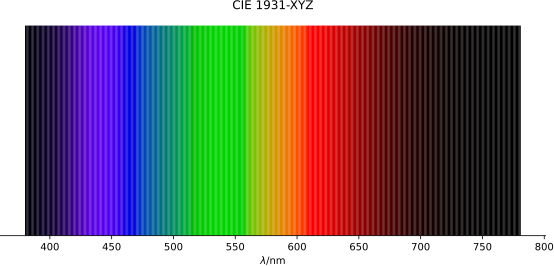
\includegraphics[width=0.65\textwidth]{"./imgs/sec2/CIE 1931-XYZ-spd.png"}
    \caption{CIE 1931-XYZ可见光谱}
    \label{fig:wave}
\end{figure}


\subsection{光谱功率分布图与分析}

\begin{figure}[htbp]
    \centering
    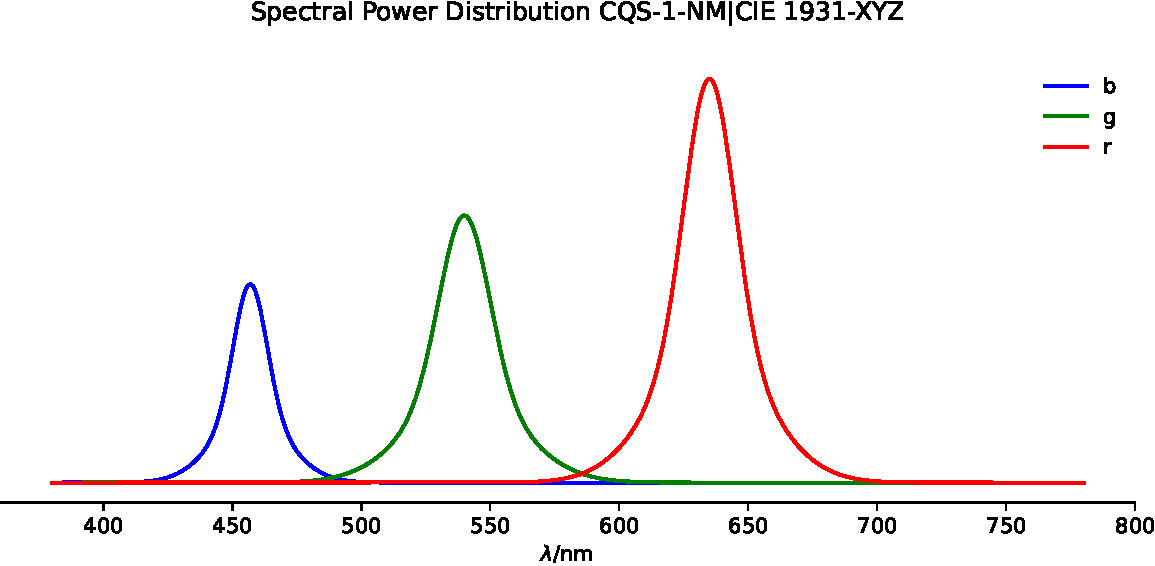
\includegraphics[width=0.65\textwidth]{"./imgs/sec2/CQS-1-NM-spd-rgb.pdf"}
    \caption{基于CIE 1931-XYZ的光谱功率分布图 -- 无背景}
    \label{fig:spd1931nobg}
\end{figure}

解决了可见光谱的问题,接下来就十分简单了,只需要录入数据,设定好波长范围与归一化的预处理(全局或者每通道归一化),画到图上即可。

本文的LED数据来源为宾夕法尼亚州立大学照明实验室(llab),具体网址可见首页脚注,本文将RGB三色数据提取出来,匹配CIE格式(txt,csv)。最终的谱功率分布图如图\ref{fig:spd1931nobg}(无背景)、图\ref{fig:spd1931bg}(未通道归一化)与图\ref{fig:spd1931bgn}(通道归一化)所示。大体操作可见于\textbf{utils/get\_spd.py}中的\textit{get\_spd}函数与\textit{spd\_background}函数。



\begin{figure}[htbp]
    \centering
    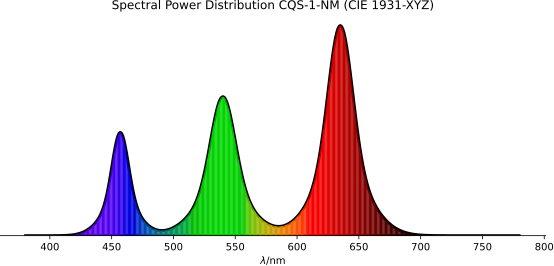
\includegraphics[width=0.65\textwidth]{"./imgs/sec2/CQS-1-NM-1931-spd.png"}
    \caption{基于CIE 1931-XYZ的光谱功率分布图}
    \label{fig:spd1931bg}
\end{figure}

\begin{figure}[htbp]
    \centering
    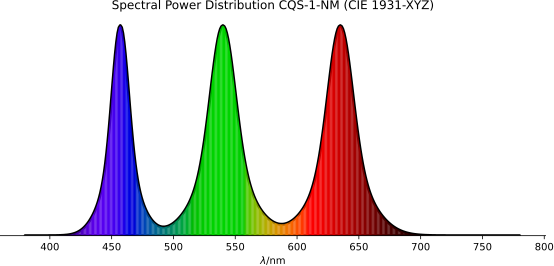
\includegraphics[width=0.65\textwidth]{"./imgs/sec2/CQS-1-NM-1931-spd-n.png"}
    \caption{基于CIE 1931-XYZ的光谱功率分布图 -- 通道归一化}
    \label{fig:spd1931bgn}
\end{figure}

如上所示,我们完成了第一个子目标,完成了光谱图的绘制。